% Figure 3: Split-at-MPP Knot Construction — Annotated J-V Curve
% Compile: pdflatex fig3_split_mpp.tex
\documentclass[border=8pt]{standalone}
\usepackage{tikz}
\usepackage{amsmath,amssymb}
\usepackage{pgfplots}
\pgfplotsset{compat=1.18}
\usetikzlibrary{
  arrows.meta,
  calc,
  positioning,
  decorations.pathreplacing,
  decorations.markings,
  patterns,
  fit,
  backgrounds,
  shadows.blur
}

\definecolor{region1}{HTML}{2980B9}
\definecolor{region2}{HTML}{E67E22}
\definecolor{curveblk}{HTML}{2C3E50}
\definecolor{anchorred}{HTML}{C0392B}
\definecolor{knotgrn}{HTML}{27AE60}
\definecolor{annotgray}{HTML}{7F8C8D}
\definecolor{mppfill}{HTML}{F39C12}
\definecolor{bgcard}{HTML}{FDFEFE}

\begin{document}
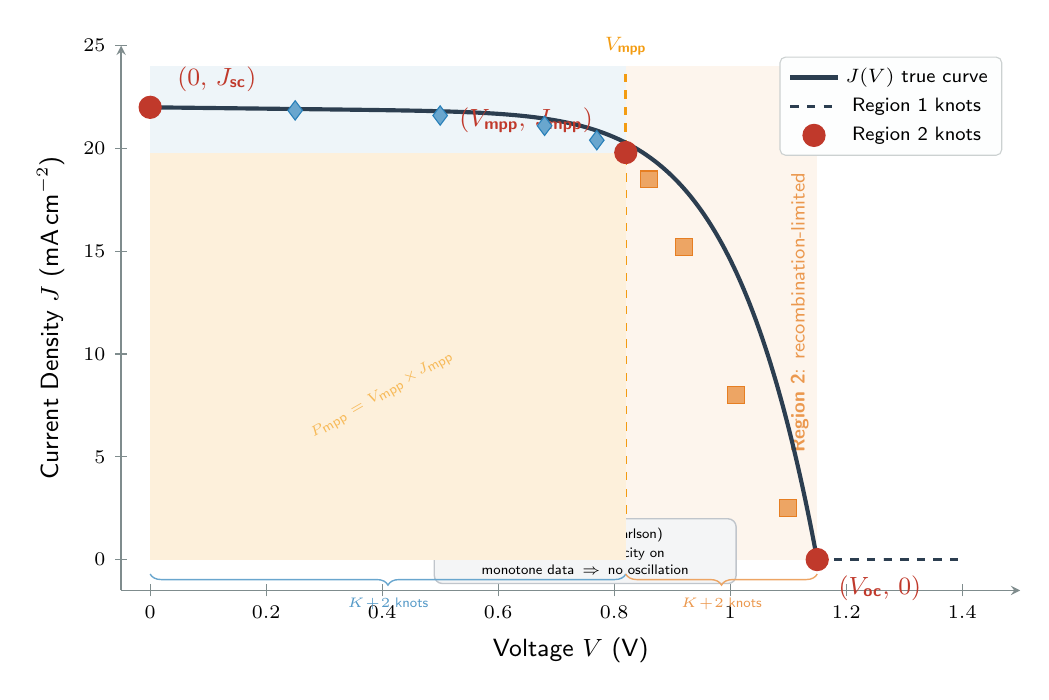
\begin{tikzpicture}

\begin{axis}[
  width=13cm,
  height=8.5cm,
  xlabel={Voltage $V$ (V)},
  ylabel={Current Density $J$ (mA\,cm$^{-2}$)},
  xlabel style={font=\sffamily\small},
  ylabel style={font=\sffamily\small},
  tick label style={font=\sffamily\scriptsize},
  xmin=-0.05, xmax=1.5,
  ymin=-1.5, ymax=25,
  axis lines=left,
  axis line style={line width=0.5pt, color=annotgray},
  every tick/.style={annotgray},
  grid=none,
  clip=false,
  legend style={
    at={(0.98,0.98)},
    anchor=north east,
    font=\sffamily\scriptsize,
    draw=annotgray!40,
    fill=bgcard,
    rounded corners=2pt,
  },
]

% ═══════════════════════════════════════════
% REGION SHADING
% ═══════════════════════════════════════════
% Region 1: transport-limited (0 → Vmpp)
\fill[region1!8] (axis cs:0,0) rectangle (axis cs:0.82,24);
% Region 2: recombination-limited (Vmpp → Voc)
\fill[region2!8] (axis cs:0.82,0) rectangle (axis cs:1.15,24);

% Region labels
\node[font=\sffamily\scriptsize, text=region1!80, rotate=90] at (axis cs:0.05,12) {
  \textbf{Region 1}: transport-limited
};
\node[font=\sffamily\scriptsize, text=region2!80, rotate=90] at (axis cs:1.12,12) {
  \textbf{Region 2}: recombination-limited
};

% MPP dividing line
\draw[mppfill, line width=1.0pt, dashed] (axis cs:0.82,-1) -- (axis cs:0.82,24)
  node[above, font=\sffamily\scriptsize\bfseries, text=mppfill] {$V_{\text{mpp}}$};

% ═══════════════════════════════════════════
% MAIN J-V CURVE (synthetic representative)
% ═══════════════════════════════════════════
% Typical perovskite J-V: Jsc ≈ 22, Voc ≈ 1.1, Vmpp ≈ 0.82, Jmpp ≈ 20
\addplot[
  curveblk,
  line width=1.5pt,
  smooth,
  samples=100,
  domain=0:1.15,
] {
  22.0 * (1 - (x/1.15)^8) * (1 - 0.015*x)
};
\addlegendentry{$J(V)$ true curve}

% Extend to zero after Voc
\addplot[curveblk, line width=1.0pt, dashed, domain=1.15:1.4] {0};

% ═══════════════════════════════════════════
% ANCHOR POINTS (large markers)
% ═══════════════════════════════════════════
% (0, Jsc)
\addplot[only marks, mark=*, mark size=4pt, anchorred, mark options={fill=anchorred}]
  coordinates {(0, 22.0)};
\node[font=\sffamily\small\bfseries, text=anchorred, anchor=south west] at (axis cs:0.03, 22.3) {
  $(0,\, J_{\text{sc}})$
};

% (Vmpp, Jmpp)
\addplot[only marks, mark=*, mark size=4pt, anchorred, mark options={fill=anchorred}]
  coordinates {(0.82, 19.8)};
\node[font=\sffamily\small\bfseries, text=anchorred, anchor=south east] at (axis cs:0.78, 20.3) {
  $(V_{\text{mpp}},\, J_{\text{mpp}})$
};

% (Voc, 0)
\addplot[only marks, mark=*, mark size=4pt, anchorred, mark options={fill=anchorred}]
  coordinates {(1.15, 0)};
\node[font=\sffamily\small\bfseries, text=anchorred, anchor=north west] at (axis cs:1.17, -0.3) {
  $(V_{\text{oc}},\, 0)$
};

% ═══════════════════════════════════════════
% INTERIOR KNOTS — Region 1
% ═══════════════════════════════════════════
% K=4 interior knots, MPP-clustered (denser near Vmpp)
% Voltage positions via clustering: ~0.25, 0.50, 0.68, 0.77
\addplot[
  only marks, mark=diamond*, mark size=3.5pt,
  region1, mark options={fill=region1!70}
] coordinates {
  (0.25, 21.85)
  (0.50, 21.6)
  (0.68, 21.1)
  (0.77, 20.4)
};
\addlegendentry{Region 1 knots}

% ═══════════════════════════════════════════
% INTERIOR KNOTS — Region 2
% ═══════════════════════════════════════════
% K=4 interior knots, MPP-clustered (denser near Vmpp)
% Voltage positions: ~0.86, 0.92, 1.01, 1.10
\addplot[
  only marks, mark=square*, mark size=3pt,
  region2, mark options={fill=region2!70}
] coordinates {
  (0.86, 18.5)
  (0.92, 15.2)
  (1.01, 8.0)
  (1.10, 2.5)
};
\addlegendentry{Region 2 knots}

% ═══════════════════════════════════════════
% ANNOTATIONS — Knot construction
% ═══════════════════════════════════════════

% Cumsum annotation box (Region 1 V-knots)
\node[
  draw=region1!50, fill=bgcard, rounded corners=3pt,
  font=\sffamily\tiny, text width=3.2cm, align=left,
  line width=0.4pt,
  anchor=north west,
] (cumsumbox1) at (axis cs:0.02, 17) {
  \textbf{$V$-knots} (Region 1):\\[1pt]
  $\sigma(\alpha^{(1)}) \xrightarrow{\text{cumsum}}$\\
  strictly $\uparrow$ in $[0, V_{\text{mpp}}]$\\[2pt]
  \textbf{$J$-knots}:\\
  $J_{\text{sc}} \to J_{\text{mpp}}$ via\\
  cumulative scaling
};

% J-monotonicity annotation (Region 2)
\node[
  draw=region2!50, fill=bgcard, rounded corners=3pt,
  font=\sffamily\tiny, text width=3.2cm, align=left,
  line width=0.4pt,
  anchor=north west,
] (cumsumbox2) at (axis cs:0.02, 9.5) {
  \textbf{$V$-knots} (Region 2):\\[1pt]
  $\sigma(\alpha^{(2)}) \xrightarrow{\text{cumsum}}$\\
  strictly $\uparrow$ in $[V_{\text{mpp}}, V_{\text{oc}}]$\\[2pt]
  \textbf{$J$-knots}:\\
  $J_{\text{mpp}} \to 0$ via\\
  cumulative scaling
};

% PCHIP callout
\node[
  draw=curveblk!30, fill=curveblk!5, rounded corners=3pt,
  font=\sffamily\tiny, text width=3.6cm, align=center,
  line width=0.5pt,
  anchor=south,
] (pchipnote) at (axis cs:0.75, -1.2) {
  \textbf{PCHIP} (Fritsch--Carlson)\\[1pt]
  preserves monotonicity on\\
  monotone data \,$\Rightarrow$\, no oscillation
};

% Brace under Region 1
\draw[
  decorate, decoration={brace, amplitude=4pt, mirror, raise=3pt},
  line width=0.5pt, region1!70
] (axis cs:0, -0.3) -- (axis cs:0.82, -0.3)
  node[midway, below=8pt, font=\sffamily\tiny, text=region1!80] {
    $K\!+\!2$ knots
  };

% Brace under Region 2
\draw[
  decorate, decoration={brace, amplitude=4pt, mirror, raise=3pt},
  line width=0.5pt, region2!70
] (axis cs:0.82, -0.3) -- (axis cs:1.15, -0.3)
  node[midway, below=8pt, font=\sffamily\tiny, text=region2!80] {
    $K\!+\!2$ knots
  };

% MPP power rectangle (subtle)
\fill[mppfill!15] (axis cs:0,0) rectangle (axis cs:0.82,19.8);
\node[font=\sffamily\tiny, text=mppfill!70, rotate=30] at (axis cs:0.40,8) {
  $P_{\text{mpp}} = V_{\text{mpp}} \!\times\! J_{\text{mpp}}$
};

\end{axis}
\end{tikzpicture}
\end{document}
